%%%%%%%%%%%%%%%%%%%%%%%%%%%%%%%% 
\section{The Data Acquisition (DAQ) System and Monitoring} 
\label{sec:detectors-fd-ref-daq}

The scope of the DAQ and monitoring includes the design, procurement,
fabrication, testing, delivery and installation. It is required to:
\begin{itemize}
\item collect data with an uptime of $>90$\%
\item collect interactions with an energy deposition of
  100\,MeV and above with a high resolution (smart or no
  zero-suppression) with no dead-time.
\item have the capability to collect interactions with an energy $<100$\,MeV with some
 low amount of zero-suppression loss.
\item have the ability to trigger at the time of the beam pulses,
  irrespective of how little energy is deposited in the detector.
\item collect data with the most favorable zero-suppression possible over a
  period of >10\,s (supernova trigger)
\item assemble data from sub-detectors into a unified
  event for offline analysis.
\item provide access to the shift operator and others to control and
  monitor the data collection and detector status, view online
  histograms and monitor (and provide for offline use) historical
  status of measured detector parameters. 
\end{itemize}
%The design presented here   AH: this sounded too bold, somehow.
This section outlines a conceptual design intended to meet the required performance for the DAQ
for the DUNE far detector. 

To dramatically 
\fixme{To reduce the deadtime of the overall DUNE detector sufficiently to meet the requirements... AH}
reduce the times when none of the parts of DUNE is
collecting data (particularly important for supernova detection) and
to allow
\fixme{dissimilar DAQ designs in each of the four 10-kt detector modules..}  the designs of the DAQ in the different 10-kt sections to be
entirely different if desired, 
\fixme{the DUNE DAQ employs the most uncoupled design to date. (but less coupled or more uncoupled to/from what?}
a less coupled design than has ever
been used in data acquisition before is employed.  The
synchronization, triggering, data collection and run-state in the
different 10-kt modules are completely independent in real time and
are only coupled by processes running asynchronously (in the same fashion
as a batch queue) in the hour or so after data collection (see section
4.11 of \anxlbnefd).  This allows one %portion of the
detector module to be restarted without interrupting data collection in the
others. %rest.

The layout of the DAQ is shown schematically in
Figure~\ref{fig:fddaqblock}.  To collect the fullest detail of the
most important events (deadtimeless detection of all those with energy
deposition of 100\,MeV and above), while avoiding tricky communication
to flag neighboring channels to those that have large hits, a model
in which the data are collected twice is used. 
\fixme{Previous sentence not clear: you want to flag channels that have large hits and NOT flag
neighboring channels?  What's the `tricky communication'?}
  The first collection
supplies a centralized software-based trigger farm continuously with
zero-suppressed information (a threshold on each channel detects hits
above the noise level; this causes the ADC samples to be kept in a
time window around the hit).  
The second pass reads the full data at the times and
in the regions %of interest that have been 
selected by the
trigger. This is similar to the triggering in a collider experiment,
but with only one level of triggering. \fixme{in other words, here we have one trigger + two collections; in collider expt, two of each? Please clarify sentence.} The software trigger farm also
records the continuous stream of zero-suppressed hits in an archival
ring buffer on disk to allow later analysis of supernova candidates.

\begin{cdrfigure}[DAQ subsystem block diagram]{fddaqblock}{Block diagram layout of the main
    components of the DAQ subsystem.}
\begin{tikzpicture}[
  every matrix/.style={ampersand replacement=\&,column sep=0.4cm,row sep=0.6cm},
  to/.style={->,>=stealth',shorten >=1pt,semithick,font=\sffamily\footnotesize},
  data/.style={thick},
%  box/.style={draw,thick,rounded corners,fill=yellow!20,inner sep=.3cm},
  box/.style={draw,inner sep=.1cm},
  boxa/.style={box,align=center}]

% Lay the nodes out using a matrix
  \matrix{   
% 1st row
  \node[boxa] (ce) {{\rm Cold}\\{\rm electronics}};
 \&
 \& \node[boxa] (rce) {{\rm RCE}\\{\rm LArTPC data}\\{\rm processors}};
 \&
 \& \node[boxa] (trigfe) {{\rm Trigger}\\{\rm frontend}\\{\rm computers}};
 \& \node[boxa] (trigbe) {{\rm Software}\\{\rm trigger}\\{\rm farm}}; \\

% 2nd row
 \& \node[box,inner sep=0.4cm] (fthru) {}; 
 \& \node[boxa] (time) {{\rm Time}\\{\rm sync}};
 \&
 \& \node[boxa] (sc) {{\rm Slow}\\{\rm control}};
 \& \\

% 3rd row
  \node[boxa] (pd) {{\rm Photon}\\{\rm detectors}};
 \&
 \& \node[boxa] (ssp) {{\rm SSP}\\{\rm Photodetector}\\{\rm digitizers}};
 \&
 \& \node[boxa] (datafe) {{\rm Data}\\{\rm frontend}\\{\rm computers}};
 \& \node[boxa] (databe) {{\rm Full-data}\\{\rm collection}\\{\rm farm}}; \\
 };

\coordinate (fthruWL) at ($ (fthru.south west)!0.3!(fthru.north west) $);   % West Low edge of fthru 
\coordinate (fthruWH) at ($ (fthru.south west)!0.7!(fthru.north west) $);   % West High edge of fthru 
\coordinate (fthruEL) at ($ (fthru.south east)!0.3!(fthru.north east) $);   % East Low edge of fthru 
\coordinate (fthruEH) at ($ (fthru.south east)!0.7!(fthru.north east) $);   % East High edge of fthru 

\coordinate (trigfeWL) at ($ (trigfe.south west)!0.3!(trigfe.north west) $);   % West Low edge of trigfe 
\coordinate (trigfeWH) at ($ (trigfe.south west)!0.7!(trigfe.north west) $);   % West High edge of trigfe
\coordinate (datafeWL) at ($ (datafe.south west)!0.3!(datafe.north west) $);   % West Low edge of datafe
\coordinate (datafeWH) at ($ (datafe.south west)!0.6!(datafe.north west) $);   % West High edge of datafe

\coordinate (rceEL) at ($ (rce.south east)!0.3!(rce.north east) $);  % East low edge of RCE 
\coordinate (rceEH) at ($ (rce.south east)!0.7!(rce.north east) $);
\coordinate (sspEL) at ($ (ssp.south east)!0.3!(ssp.north east) $);  % East low edge of SSP
\coordinate (sspEH) at ($ (ssp.south east)!0.8!(ssp.north east) $);

\coordinate (rceSR) at ($ (rce.south)+(0.7cm,0) $);  % South right edge of RCE 
\coordinate (sspNR) at ($ (ssp.north)+(0.7cm,0) $);  % North right edge of RCE 
\coordinate (scWL) at ($ (sc.south west)!0.3!(sc.north west) $);  % West low edge of SC 
\coordinate (scWH) at ($ (sc.south west)!0.7!(sc.north west) $);  % West high edge of SC 

\draw[data] (ce) -| ($(fthruWH)-(0.1cm,0)$) -- (fthruWH);
\draw[data] (pd) -| ($(fthruWL)-(0.1cm,0)$) -- (fthruWL);
\draw[data] (fthruEH) -- ($(fthruEH)+(0.1cm,0)$) |- (rce);
\draw[data] (fthruEL) -- ($(fthruEL)+(0.1cm,0)$) |- (ssp);

\draw[data] (rceEH) -- ($ (rceEH)+(0.40cm,0) $) |- (trigfeWH); 
\draw[data] (rceEL) -- ($ (rceEL)+(0.40cm,0) $) |- (datafeWH); 
\draw[data] (sspEH) -- ($ (sspEH)+(0.55cm,0) $) |- (trigfeWL); 
\draw[data] (sspEL) -- ($ (sspEL)+(0.55cm,0) $) |- (datafeWL); 

\draw[data] (trigfe) -- (trigbe);
\draw[data] (datafe) -- (databe);

\draw[data,dashed] (time) -- (rce);
\draw[data,dashed] (time) -- (ssp);

\draw[data,dashed] (scWH) -| (rceSR);
\draw[data,dashed] (scWL) -| (sspNR);

\draw[data,dotted] (fthru.north) -- ($(fthru.north)+(0,2.7cm)$) node [left] {\rm In cryostat} node [right] {\rm Room temp.};
\draw[data,dotted] (fthru.south) -- ($(fthru.south)-(0,2.7cm)$);
\end{tikzpicture}
\end{cdrfigure}

{\bf LArTPC detector readout} The LArTPC signals are digitized in a
continuous flash-ADC stream at 2\,MHz, (not zero-suppressed) and
serialized on 12,000 high-speed links per 10-kt module that exit the
cryostat (costed separately in the cold-electronics WBS). \fixme{Do we want to refer to costs here?
And which thing falls under CE, the links? Maybe say `(the links are covered in Section~\ref{sec:detectors-fd-ref-ce})'} The data
are received by RCE LArTPC data processors %which are 
housed in
industry-standard aTCA crates on COB boards that are designed at SLAC
for a wide range of applications.  The RCEs are part of a network of
field programmable gate arrays (FPGAs) that buffer the full raw data,
zero-suppress it for passing to the trigger and accept requests for
data-fetching from the trigger.  The FPGAs in the RCEs are from the
Xilinx Zynq family and contain a full Linux processor system on the
chip.  They facilitate the high-speed data transfer from firmware into
DRAM memory that is accessible from Linux.  A fast data-transfer
network using the Ethernet protocol is used on the COBs and in the
aTCA crates to allow for deveopment of more sophisticated zero-suppression algorithms
for improved supernova acquisition.

{\bf Photon detector readout} is costed separately in the photon
detector WBS, the SSP modules amplify and supply bias voltages,
assemble and process a waveform at 128\,MHz for each hit which is
detected.\fixme{Continue with this (AH: Why can't you just say `Photon detector readout is covered
in Section~\ref{detectors-fd-ref-pd}? }.

{\bf Computer farm} Both the LArTPC and photon detector data are
received in commodity Linux computers, with no deadtime, from where
the data are routed to the trigger and full-data collection farms of
computers.  Although the front-end computers are logically distinct as
shown in Figure~\ref{fig:fddaqblock}, one physical computer is
sufficient for all the processes for each rack of APA readout
electronics.

{\bf artDAQ software toolkit} (from Fermilab) supplies the real-time
data collection functionality (buffering, matching event parts,
synchronization, inter-process communication, etc.) in a modern C++11
code design that facilitates the efficient use of multicore commodity
computers running on the Linux computer farms.  The detector-specific
code is supplied by DUNE groups (this is centered in the UK), along
with detector-specific triggering (also UK).  The architecture
provided by artDAQ can be tailored for each experiment and is entirely
suitable for the ``collect-twice'' architecture envisioned for DUNE.

{\bf Run Control and Slow Control software framework} manages the
control, status display and status archival of the experiment.  This
exploits a combination of readily available, well-supported packages
[message passing (zeroMQ), a web-framework (Django), databases
(postgress)] to give the shift operator a unified view of the status
of the running experiment, and views of the monitoring data including
customized views and historical views.  The database of slow-control
measurements is exported to the host lab to give access for offline
programs.

{\bf Timing system} To acomplish the software-based deadtimeless data
acquisition in DUNE, it is necessary to synchronize the clock across
all readout boards.  This is accomplished in two stages, the main
cavern-wide distribution uses the design from the NO$\nu$A experiments
which distributes a 64-MHz clock, synchronization pulses and
cable-delay correction on RJ45 cables.  The overall clock is
synchronized using a GPS receiver and transferred from the surface
over optical fiber.  The synchronization is transferred from the COBs
to the electronics in the cryostat over the same cabling as provides
the data links.

{\bf Calibration system} The calibration is done in three stages: (1)
Pedestal and charge-injection pulser events are used to calibrate and
remove drifting of the individual electronic channel responses. (2)
External UV lasers are directed into the cryostat through glass-tube
ports, and swivelling mirrors select the trajectories of the beams
through the cryostat to provide calibration of the field
non-uniformities and attenuation. (3) Cosmic-ray muons are used for
the determination of the energy scale and for calibration
cross-checks.

\begin{cdrfigure}[DAQ time diagram]{fddaqtime}{Main DAQ steps displayed relative to the event time.}
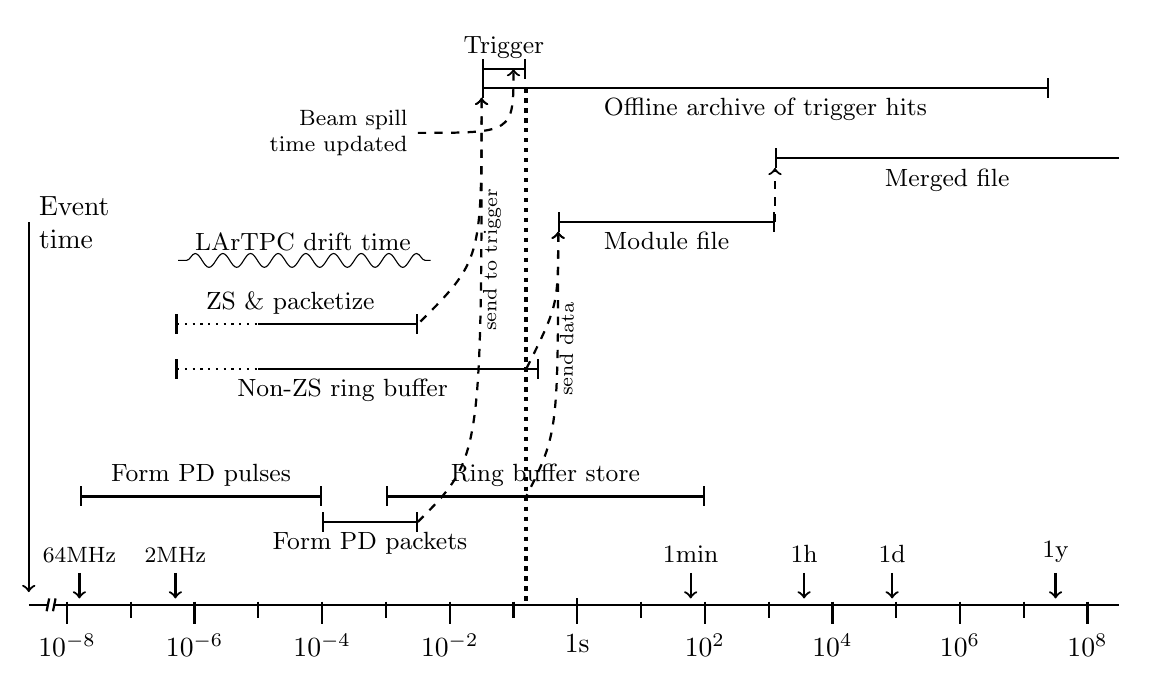
\begin{tikzpicture}[scale=0.81,
  every matrix/.style={ampersand replacement=\&,column sep=0.4cm,row sep=0.6cm},
  to/.style={->,>=stealth',shorten >=1pt,semithick,font=\sffamily\footnotesize},
  timeline/.style={thick},
  transline/.style={dashed,thick},
  pointline/.style={thick},
  proline/.style={thick},
  driftline/.style={shorten <=1pt,decorate,decoration={snake,pre length=4pt}},
  data/.style={thick},
%  box/.style={draw,thick,rounded corners,fill=yellow!20,inner sep=.3cm},
  box/.style={draw,inner sep=.1cm},
  boxa/.style={box,align=center}]

\draw [timeline] (-8.2,0) -- (8.5,0);
\foreach \i in {-8,-6,-4,-2,2,4,6,8}
  \draw [timeline] (\i,0.05) -- (\i,-0.3) node [below] {$10^{\i}$};
\foreach \i in {-7,-5,-3,-1,1,3,5,7}
  \draw [timeline] (\i,0.05) -- (\i,-0.2);
\draw [timeline] (0,0.1) -- (0,-0.3) node [below] {$1\mathrm{s}$};

\draw [pointline,->] (-8.6,6) node [right,align=left] {{\rm Event}\\{\rm time}} -- (-8.6,0.2);
\draw [timeline] (-8.6,0) -- (-8.3,0);
\draw [timeline] (-8.28,0.1) -- (-8.32,-0.1);
\draw [timeline] (-8.18,0.1) -- (-8.22,-0.1);

\draw [pointline,->] (1.77815,0.5) node [above,font=\small] {\rm 1min} -- (1.77815,0.1);
%\draw [pointline,->] (2.77815,-0.9) node [anchor=north] {$10\mathrm{m}$} -- (2.77815,-0.1);
\draw [pointline,->] (3.5563,0.5) node [above,font=\small] {\rm 1h} -- (3.5563,0.1);
%\draw [pointline,->] (4.5563,-0.9) node [anchor=north] {$10\mathrm{h}$} -- (4.5563,-0.1);
\draw [pointline,->] (4.9365,0.5) node [above,font=\small] {\rm 1d} -- (4.9365,0.1);
\draw [pointline,->] (7.4988,0.5) node [above,font=\small] {\rm 1y} -- (7.4988,0.1);

\draw [pointline,->] (-7.8061,0.5) node [above,font=\footnotesize] {\rm 64MHz} -- (-7.8061,0.1);
\draw [proline,|-|] (-7.8,1.7) -- node [above,font=\small] {\rm Form PD pulses} (-4,1.7);
\draw [proline,|-|] (-4,1.3) -- node [below,font=\small] {\rm Form PD packets} (-2.5,1.3);
\draw [proline,|-|] (-3,1.7) -- node [above,font=\small] {\rm Ring buffer store} (2,1.7);

\draw [driftline] (-6.3,5.4) -- node [above,font=\small] {\rm LArTPC drift time} (-2.3,5.4);

\draw [pointline,->] (-6.3010,0.5) node [above,font=\footnotesize] {\rm 2MHz} -- (-6.3010,0.1);
\draw [proline,|-,dotted] (-6.3010,4.4) -- (-5,4.4);
\draw [proline,-|] (-5,4.4) -- node [above,pos=0.2,font=\small] {\rm ZS \& packetize} (-2.5,4.4);
\draw [proline,-|] (-5,3.7) -- node [below,pos=0.3,font=\small] {\rm Non-ZS ring buffer} (-0.6,3.7);
\draw [proline,|-,dotted] (-6.3010,3.7) -- (-5,3.7);

\draw [transline,<-] (-1.5,7.95) .. controls (-1.5,5.4) .. node [below,sloped,pos=0.35,font=\scriptsize] {} (-2.5,4.4);  
\draw [transline,<-] (-1.5,7.95) .. controls (-1.5,2.3) .. node [below=-3pt,sloped,pos=0.18,font=\scriptsize] {\rm send to trigger} (-2.5,1.3);  
\draw [transline,->] (-2.5,7.4) node [anchor=east,align=right,font=\footnotesize] {{\rm Beam spill}\\{\rm time updated}}.. controls (-1.0,7.4) .. (-1.0,8.4);  
\draw [proline,|-|] (-1.5,8.4) -- node [above,font=\small] {\rm Trigger} (-0.8,8.4);
\draw [proline,|-|] (-1.5,8.1) -- node [below,font=\small] {\rm Offline archive of trigger hits} (7.4,8.1);

\draw [dotted,ultra thick] (-0.8,8.1) node [right,font=\small] {} -- (-0.8,0.);

\draw [proline,|-|] (-0.3,6.) -- node [below,font=\small] {\rm Module file} (3.1,6.);
\draw [proline,|-] (3.1,7.) -- node [below,pos=0.5,font=\small] {\rm Merged file} (8.5,7.);
\draw [transline,->] (3.1,6.) -- (3.1,6.85);

\draw [transline,<-] (-0.3,5.85) .. controls (-0.3,2.7) .. node [below=-3pt,sloped,pos=0.25,font=\scriptsize] {\rm send data} (-0.8,1.7);  
\draw [transline,<-] (-0.3,5.85) .. controls (-0.3,4.7) .. node [above,sloped,pos=0.5,font=\small] {} (-0.8,3.7);  

\end{tikzpicture}
\end{cdrfigure}

The time sequence, trigger deadlines and buffering of the readout are all
shown in Figure~\ref{fig:fddaqtime}.  This figure shows time in the
horizontal direction on a logarithmic scale to indicate how long after
the particles appear in the detector each process can start and must
finish.  There is one level of triggering, with a trigger deadline of
0.16\,s after the event has occurred, indicated by the vertical dotted
line.  This is long enough that in 99\% of the cases, a message will
arrive from the Fermilab site to update the predicted time of a
neutrino spill with the actual time in order that the detector can be
triggered independently of any signals in the detector.  This
operation has been used succesfully on MINOS for many years.  

As shown in Figure~\ref{fig:fddaqtime}, prior to the trigger time and
independently in each detector module, the detector readout assembles
packets of data corresponding to fixed time intervals and sends them
to the trigger event builders.  Both the LArTPC readout and the SSP
readout send zero-suppressed data, suitable for triggering, to a set
of event-builder processes that run in parallel, each accepting all
the data from the entire 10-kt module for a specific time interval and
performing trigger algorithms on them.  All time intervals are
processed so that the trigger has no dead time.  The LArTPC and SSP
data also store data in ring buffers
\fixme{data store data? The lartpc and ssp somethings also store data...}
  to await collection after an
affirmative trigger decision --- in the case of the LArTPC, this data
is not zero suppressed.  The data are built into events in a ``10kt-module
file'' that is written to disk.  About an hour later, an offline process merges
the data from the separate 10-kt module files and archives them at the host lab.

To maximize data collection for a supernova, the continuous
zero-suppressed trigger data is kept in a large buffer area on disk.
Ways to collect data that is cropped more gently than the zero-suppressed 
data stream during the extended period of a supernova are
under study: The non-zero-suppressed ring buffers on the RCEs are
sufficient for 0.4\,s of buffering and the trigger farm can manage its optimal
usage during a supernova. Two possible extensions
are (a) extend the memory in the aTCA crate to buffer longer with
local disk drives, or (b) use the powerful intercommunications between
RCEs to cause neighboring channels to be kept around the time of a
potential supernova event candidate. 

\todo{DAQ2} Add table of rates and describe it.

\todo{DAQ3} Add short paragraph of assumptions made in costing etc. \fixme{I think that should go with the costing information; that's how we did it last time. TBD}

%Here is a sample table:
%
%%\begin{cdrtable}[short]{cc}{label}{long}  %The third argument (reads {cc}) can use c, l, r or p{some length} 
% but please do not include lines like “|c|l|l|”. It CAN look like {cll} or {llp{3cm}}, for instance.
%Header Column1 & Header Column 2 \\ \toprowrule
%Row 1 & First \\ \colhline
%Row 2 & Second \\ \colhline
%Row 3 & Third \\
%\end{cdrtable}
%
%Here is a sample reference to a table Table~\ref{tab:label}).  Notice: ``tab:'' is not present in the label as written in the table code itself.
